\documentclass[aspectratio=169,12pt]{beamer}
\usepackage[T1]{fontenc}
\usepackage[utf8]{inputenc}
\usepackage{lmodern}
\usepackage[spanish]{babel}
\usepackage{graphicx}
\usepackage{tikz}
\usetikzlibrary{positioning}

% Paleta neutra: gris oscuro y azul petróleo
\definecolor{gris}{HTML}{2F3A40}
\definecolor{grisclaro}{HTML}{9AA5AB}
\definecolor{petroleo}{HTML}{1F6672}
\definecolor{fondo}{HTML}{EEF2F3}

\usetheme{default}
\setbeamertemplate{navigation symbols}{}
\setbeamercolor{normal text}{fg=gris}
\setbeamercolor{frametitle}{fg=petroleo}
\setbeamercolor{title}{fg=petroleo}
\setbeamercolor{structure}{fg=petroleo}
\setbeamerfont{frametitle}{series=\bfseries,size=\LARGE}
\setbeamertemplate{frametitle}{\vspace*{0.6em}\insertframetitle\par\vspace{-0.2em}{\color{petroleo}\rule{3cm}{1.2pt}}}
\setbeamertemplate{footline}{\hfill{\color{grisclaro}\scriptsize\insertframenumber}\hspace*{1.2em}\vspace*{0.8em}}

\newcommand{\frente}[2]{%
    \begin{beamercolorbox}[wd=\linewidth,sep=7pt,rounded=false]{bloque}
      {\color{petroleo}\bfseries #1}\par\vspace{0.2em}\small #2
    \end{beamercolorbox}}

\newcommand{\fuente}[1]{\par\vfill{\color{grisclaro}\scriptsize #1}}

\title{Contabilidad de la muerte: por qué una reforma fiscal pequeña no basta}

\begin{document}

% ---------- 1. Portada ----------
\begin{frame}[plain]
  \vspace*{1.2em}
  {\color{petroleo}\bfseries\fontsize{24}{29}\selectfont Contabilidad de la muerte:\\[0.2em]
  por qué una reforma fiscal pequeña no basta\par}
  \vspace{0.4em}{\color{petroleo}\rule{4cm}{1.5pt}}\par
  \vspace{1.2em}
  {\large\bfseries Héctor Juan Villarreal Páez\par}
  {\normalsize Escuela de Gobierno y Transformación Pública, Tecnológico de Monterrey\par}
  \vspace{1.4em}
  {\small Foro «Política hacendaria: los límites del presente y las posibilidades del futuro»\\
  Panel Gastos e Ingresos\\
  Organizan: Pensando en México · La Fuerza Naranja\\[0.5em]
  13 de octubre de 2026\par}
\end{frame}

% ---------- 2. Punto de partida ----------
\begin{frame}{El punto de partida}
  \begin{columns}[c]
    \begin{column}{0.58\textwidth}
      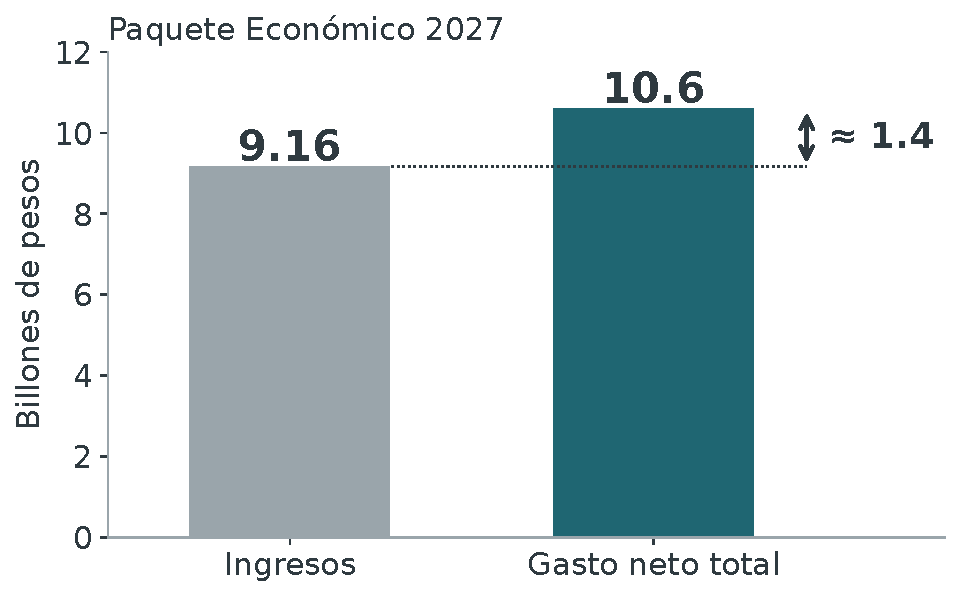
\includegraphics[width=\linewidth]{fig/l2_ingresos_gasto_2027.pdf}
    \end{column}
    \begin{column}{0.38\textwidth}
      \Large En 2027 el gasto supera a los ingresos por
      {\color{petroleo}\bfseries $\approx$\,1.4 billones} de pesos.
    \end{column}
  \end{columns}
  \fuente{Paquete Económico 2027. Fuente: elaboración propia con datos de CIEP (2026), \emph{Implicaciones del Paquete Económico 2027}, con información de SHCP.}
\end{frame}

% ---------- 3. Contabilidad de la muerte ----------
\begin{frame}{De cada peso, casi todo ya tiene dueño}
  \centering
  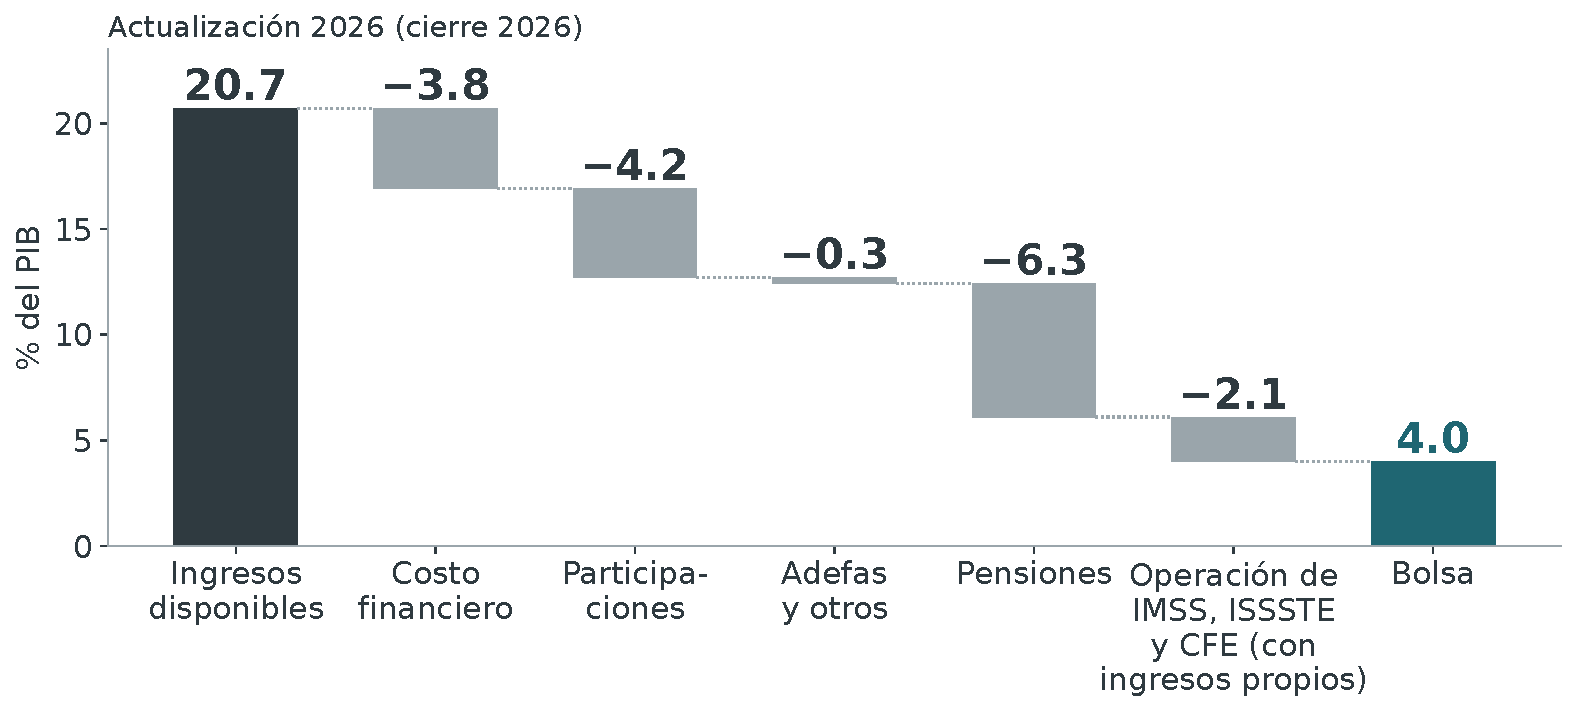
\includegraphics[width=0.82\textwidth]{fig/l3_cascada_2026.pdf}\par
  \vspace{0.1em}
  {\small Sin petroleros: transferencias del FMP (0.7) y apoyos a Pemex (0.7) se compensan.\par}
  \fuente{Supuestos generosos con la SHCP (PIB nominal 2026 de 36,500 mmdp); la bolsa real probablemente es menor. Actualización 2026.
  Fuente: elaboración propia con datos de SHCP (enero--julio 2026, cifras anuales estimadas).}
\end{frame}

% ---------- 4. Todo compite por la Bolsa ----------
\begin{frame}{Todo compite por la Bolsa}
  \begin{columns}[c]
    \begin{column}{0.52\textwidth}
      \centering
      \begin{tikzpicture}
        \node[draw=petroleo, line width=1.5pt, fill=fondo, rounded corners=4pt,
              minimum width=6.4cm, minimum height=3.9cm, align=center, text=gris] (b) {
          {\color{petroleo}\bfseries\LARGE 4.0\,\% del PIB}\\[0.6em]
          Salud · Educación\\[0.2em]
          Seguridad · Infraestructura\\[0.2em]
          Agua · Ciencia y tecnología\\[0.2em]
          Inversión pública};
      \end{tikzpicture}\par
      \vspace{0.6em}
      \normalsize Recomponer el gasto es {\color{petroleo}\bfseries repartir la escasez}.
    \end{column}
    \begin{column}{0.44\textwidth}
      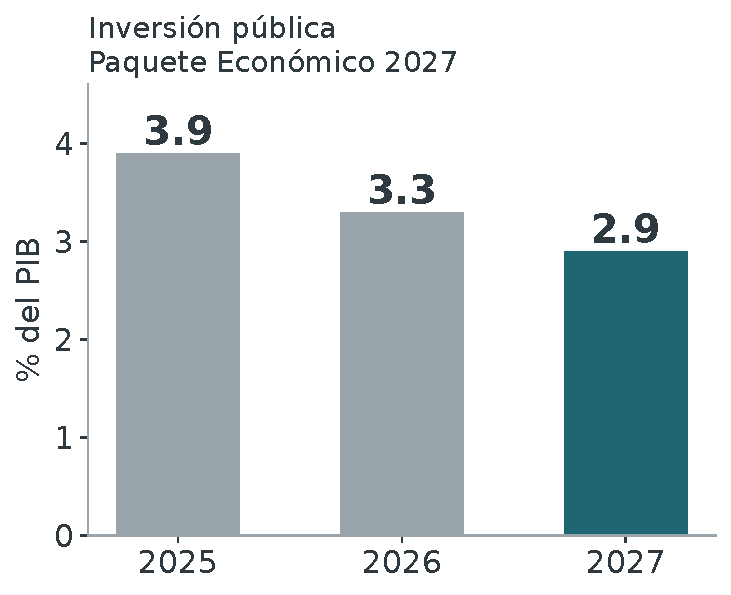
\includegraphics[height=0.62\textheight]{fig/l4_inversion_2027.pdf}
    \end{column}
  \end{columns}
  \fuente{Bolsa: actualización 2026, elaboración propia con datos de SHCP. Inversión: Paquete Económico 2027; fuente: CIEP (2026) con información de SHCP.}
\end{frame}

% ---------- 5. Una reforma pequeña no basta ----------
\begin{frame}{Una reforma pequeña no basta}
  \begin{columns}[c]
    \begin{column}{0.58\textwidth}
      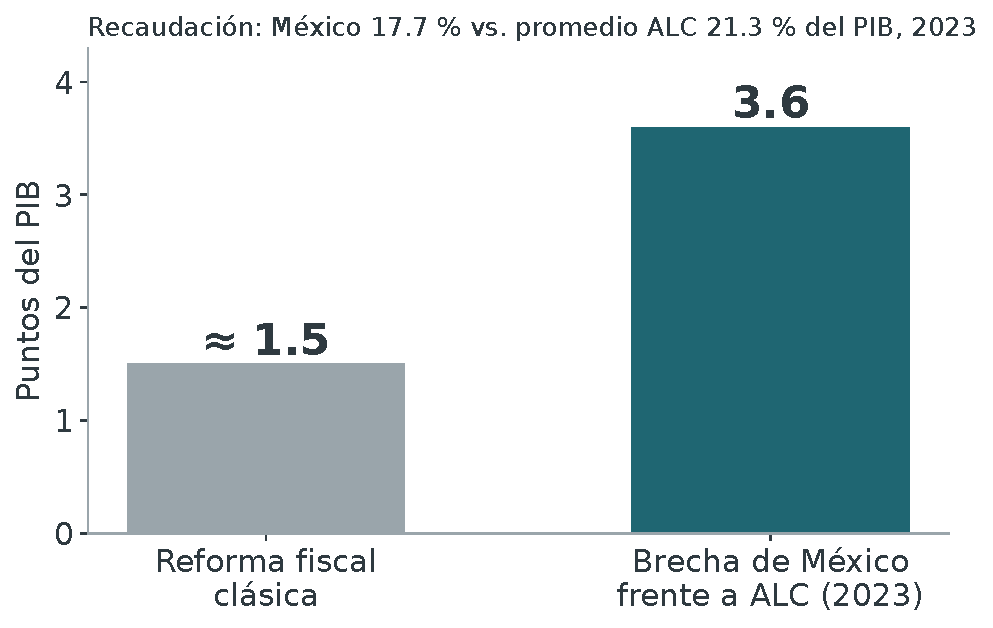
\includegraphics[width=\linewidth]{fig/l5_reforma_brecha.pdf}
    \end{column}
    \begin{column}{0.38\textwidth}
      \Large Una reforma fiscal clásica cubre
      {\color{petroleo}\bfseries menos de la mitad} de la brecha.
    \end{column}
  \end{columns}
  \fuente{Reforma clásica: del orden de 1.5 puntos del PIB. Brecha: OCDE, CEPAL, CIAT y BID (2026), \emph{Estadísticas tributarias en América Latina y el Caribe}, datos 2023, citado por CIEP (2026).}
\end{frame}

% ---------- 6. Cuatro frentes ----------
\begin{frame}{Cuatro frentes y una decisión}
  \vspace{0.3em}
  \setbeamercolor{bloque}{bg=fondo,fg=gris}
  \begin{columns}[T]
    \begin{column}{0.48\textwidth}
      \frente{Reforma fiscal clásica (federal)}{Bases gravables, gastos fiscales, IVA, ISR.}\par\vspace{0.6em}
      \frente{Haciendas locales}{Ingresos propios de estados y municipios (predial, tenencia moderna) y financiamiento de sus funciones.}
    \end{column}
    \begin{column}{0.48\textwidth}
      \frente{Seguridad social}{Pensiones y salud con financiamiento sostenible e inclusión de trabajadores informales.}\par\vspace{0.6em}
      \frente{Empresas del Estado}{Pasivos contingentes de Pemex y CFE fuera del presupuesto corriente.}
    \end{column}
  \end{columns}
  \vfill
  \setbeamercolor{banda}{bg=petroleo,fg=white}
  \begin{beamercolorbox}[wd=\textwidth,sep=10pt,center]{banda}
    \bfseries La decisión no es una medida, es un replanteamiento integral:\\
    ninguno de los cuatro frentes cierra la cuenta por sí solo.
  \end{beamercolorbox}
  \vspace*{-0.6em}
\end{frame}

\end{document}
